\section{Introduction}
\label{sect:intro}


%\textit{\textcolor{blue}{\hl{Cettina: primo draft }}}

\cettina{potremmo ridurre, ma lascerei qui la descrizione generale di ASTRI-Horn e di UVscope, mantenendo nei paragrafi successivi, come gia fatto in parte, le caratteristiche inerenti lo stato del sistema nel periodo in esame: degradazione degli specchi, condizioni meteo avverse, ecc ecc. In tal caso, il titolo del par.2 andrebbe modificato ...}

The most successful detection technique in the search for very high energy (greater than 100GeV) cosmic gamma-ray sources is the observation from ground of the Cherenkov light generated by secondary particle showers in the atmosphere \citep{Ong1998}. On such a technique are based the Imaging Atmospheric Cherenkov Telescopes (IACTs), large optical reflectors which concentrate Cherenkov light onto a multi-pixel photomultiplier camera. Images of the shower in one or several telescopes are analysed to reconstruct primary gamma-ray parameters.

During observations, the camera pixels are illuminated by a significant amount of Night Sky Background (NSB) light which largely dominates over the electronic noise. The NSB light depends on the region of observation and is a measure of the background noise from which the Cherenkov signals must be discerned, operation generally performed applying tailored cleaning procedures whose tail cuts are based on the knowledge of the NSB level. In general, the NSB conditions cannot be considered constant during an observation; they change more or less rapidly due to rotation of the field of view and to variation of the environmental and atmospheric conditions. It is therefore a good practice to evaluate the NSB level directly from the observation data: moreover, the knowledge of the actual NSB rate in each pixel, possibly influenced by a star in its field of view, allows to judge if a pixel can be included in the Cherenkov signal image analysis.

As for all IACTs, the problem to correctly evaluate the NSB level is present in the ASTRI-Horn telescope, which this article refers to. The telescope, named ASTRI-Horn in honor of the Italian-Jewish astronomer Guido Horn D'Arturo, who pioneered the use of segmented primary mirrors in astronomy \citep{Horn}, is located on Mt. Etna, Serra La Nave, Italy, at the INAF "M.C. Fracastoro" observing station (37.7$^{\circ}$N, 15.0$^{\circ}$E, 1740~m a.s.l.)
equipped with various instrumentation for the monitoring of meteorological and environmental conditions \citep{Maccarone2013}. A complete description of the ASTRI-Horn telescope can be found in several contributions and references therein (see \citep{Lombardi2020} for a comprehensive bibliography); here we recall its basic features.

\begin{figure}
\centering{
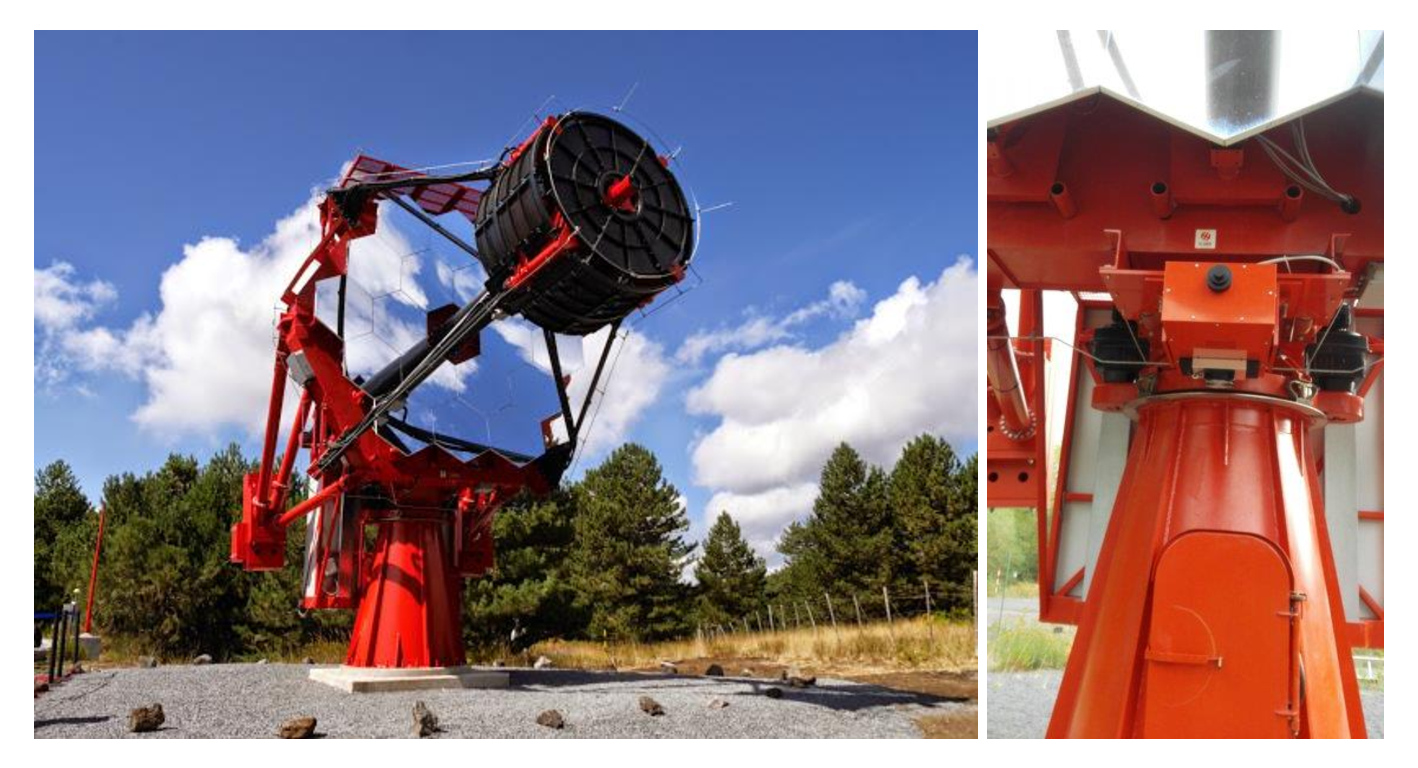
\includegraphics[width=12cm]{Figure/ASTRI-Horn-with-UVscope}}
\caption{ASTRI-Horn, the dual-mirror Cherenkov telescope installed on Mt.Etna, Italy, at the INAF "M.C. Fracastoro" observing station. On the rigth panel it is visible the small UVscope instrument mounted under the primary mirror structure of the ASTRI-Horn telescope.}
\label{fig:ASTRI-Horn-with-UVscope}
\end{figure}

The ASTRI-Horn telescope (see Fig.\ref{fig:ASTRI-Horn-with-UVscope}) is characterized by a dual-mirror Schwarzschild-Couder optical design with a 4.3~m diameter primary mirror segmented in 18 hexagonal tiles and a monolithic 1.8~m diameter secondary mirror. The optical point spread function (PSF), defined as the 80\% of the light collected from a point like source, is contained in less than one camera pixel (0.19$^{\circ}$ angular size) over all field of view (FoV)  \citep{Giro2017}. The mirrors of the telescope dishes focus on the Cherenkov camera the Cherenkov light emitted during the development of the extensive air showers induced by the interaction of the primary cosmic-rays and VHE gamma rays with the atmosphere. The ASTRI-Horn Cherenkov camera \citep{Catalano2018}, whose sensors are Silicon Photomultipliers (SiPMs) organized in photon detection modules (PDMs), includes lodging for 37 units (currently, 21 units out of 37 are implemented in the ASTRI-Horn camera for a total effective FoV of about 7.6$^{\circ}$). The PDMs are lodged in a curved focal plane and the overall focal surface is protected from the external atmospheric environment by an optical-UV transparent poly methyl methacrylate (PMMA)  window. The PDMs  
are managed by a fast electronics system based on a peak-detector technique. The camera trigger is a topological one, activated when a given number of contiguous pixels, within a PDM, present a signal above a given threshold. The camera electronics comprises the Front-End Electronics Board (FEE) and the FPGA Board that, among other many functions, convert the analog SiPM signals into digital signals, and the Back-End Electronics (BEE) that controls and manages the overall system and provides the needed functions to process and transmit the images, as produced by the FEE, to the camera data acquisition system. The camera includes a fiber-optics calibration tool and the entire system is protected by a lid mechanism. The telescope uses an Alt-Az mount to support and point the optical system and the scientific instrumentation at any target in the part of the sky accessible from the site. On the rear of the secondary mirror support structure it is installed a Pointing Monitoring Camera (PMC) to obtain, with an accuracy of 5 arcsec over the full sky, the astrometric calibrated FoV of the region pointed to by the telescope. Beside the PMC, a Sky Quality Meter (SQM), sensitive only to visual light, is installed to measure the integral sky brightness (mag/arcsec$^{2}$) in a region of 10$^{\circ}$ around the optical axis of the telescope. All configuration and housekeeping data of the ASTRI-Horn system are stored in the Telescope Monitoring and Configuration Data Base, TMCDB, together with the data coming from the weather station and all sky camera installed at the Serra La Nave site.

As further support to the knowledge of the night sky conditions, the UVscope instrument is mounted on the external structure of the ASTRI-Horn telescope, as shown in Fig. and co-aligned with the ASTRI-Horn camera axis. UVscope is a light detector working in Single Photon Counting (SPC) mode that keep negligible the electronic noise. The instrument has been developed at INAF/IASF-Palermo and it is mainly devoted to the measurement of the NSB light and atmosphere transparency in the UV energy region (300-650 nm) \citep{Maccarone2011}. UVscope basically consists of: a photon detector with its front-end and data acquisition electronics units, and a disk emulator interface card for computer connection; a pinhole collimator to regulate the angular aperture of the detector and to protect its sensitive area against stray light; a motorized diaphragm to open/close the entrance pupil during night/day; an air-ventilation system; the power unit. To be operative, the UVscope instrument aboard ASTRI-Horn simply needs a 24 V power and an Ethernet connection (see \citep{Maccarone2020} for a detailed description of the entire apparatus).The UVscope light sensor is a Multi Anode Photo Multiplier Tube (MAPMT) manufactured by Hamamatsu, series R7600-03-M64 and calibrated according to the NIST standards. This MAPMT allows moderate imaging properties with its 64 anodes arranged in a matrix of 8${\times}$8 pixels. UVscope acquires data simultaneously with the ASTR-Horn camera, pointing the same sky region and without any interference with the main telescope.  To relate the UVscope measurements as much as possible with the central zone of the ASTRI-Horn camera, a collimator equipped with a 2~mm${\times}$2~mm entrance pupil has been used; the  distance between pupil and photocathode has been settled at 238.1~mm so to achieve an angular aperture of UVscope pixel of  0.55$^{\circ}$. Under these geometrical conditions, the UVscope field of view covers the internal area of about 3${\times}$3 PDMs of the ASTRI-Horn camera, being the aperture of each UVscope pixel equal to about 3${\times}$3 pixels of the ASTRI-Horn camera (0.19$^{\circ}$ angular pixel size), as schematized in Fig.\ref{FoV-UVscope-ASTRI}.

\begin{figure}[htb]
\begin{center}
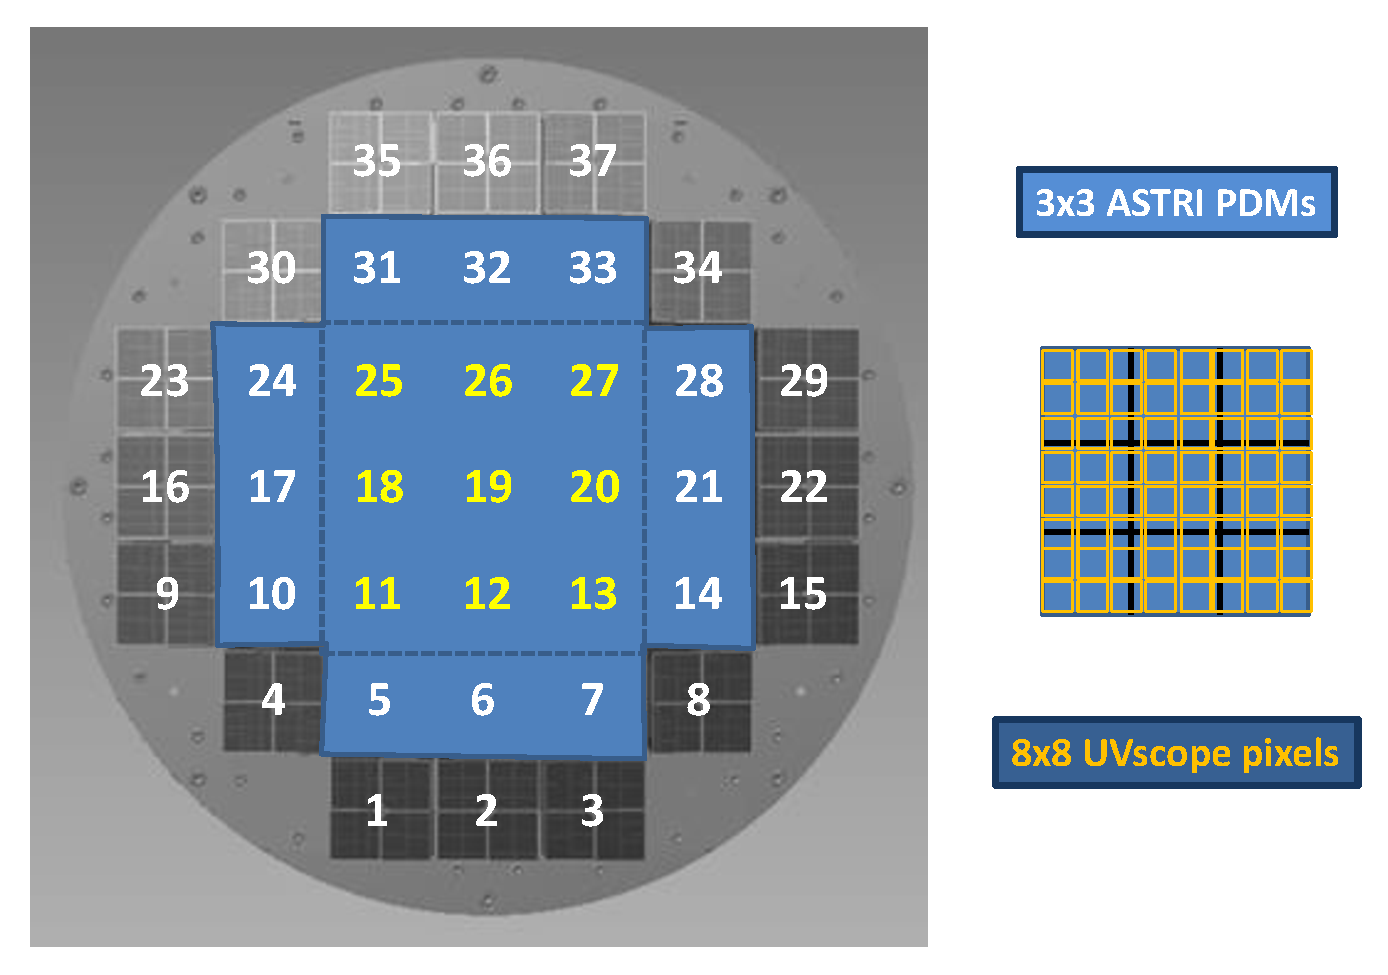
\includegraphics[width=11cm]{Figure/FoV-UVscope-ASTRI.pdf}
\caption{The ASTRI-Horn camera and UVscope dimensional correspondence.\cettina{questa figura ha risoluzione maggiore della seguente; se scegliamo questa, la caption va ancora aggiornata ...}}
\label{FoV-UVscope-ASTRI}
\end{center}
\end{figure}

\cettina{ancora da scrivere ... La base dovrebbe essere la valutazione della correlazione tra le misure di NSB diffuso ottenute da UVscope e quanto ricavato dalla analisi dei dati della camera di ASTRI-Horn}

Aim of this contribution .....

